\documentclass[a4paper,11pt]{article}

\usepackage{graphicx}
\usepackage{float}
\usepackage{listings}
\usepackage[colorlinks]{hyperref}
\title{PowerEnjoy - Design Document}
\begin{document}

\begin{titlepage}
\begin{figure}
	\centering
	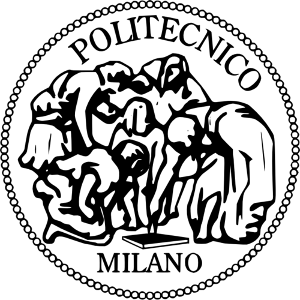
\includegraphics[width=0.5\textwidth]{images/polimi}
\end{figure}
\maketitle
\centering
A.Y. 2016/2017

Bolshakova Liubov, matr. 876911 

Gao Xiao, matr. 876265 

Kang Shuwen, matr. 876245

\end{titlepage}

\tableofcontents
\newpage
	
\section{INTRODUCTION}
	\subsection{Purpose}
	 Our team is focus on specifying the accomplishment of the service \textsl{PowerEnJoy}, this is a system which supply the electric cars to facilitate the transportation of citizens. In particular, the \textsl{PowerEnJoy} will offer the accessible electric cars in the reachable areas in the city and assign them rationally to users; the system also set rider clauses to standardize the driving behaviours of users by provide discounts and add compensations.
	 
	 This document aims to :
	 \begin{itemize}
	 \item Describe the software and hardware architecture of the system we build in the design part.
	 \item Make some reasonable adjust based on the design part, improve the system model into a more realizable direction.
	 \item Focus on the technical approach on the system realization; analyze the deep level about the algorithm.
	 \item Draw a clearer blueprint not only on the interface aspect but also on the use interaction.
	 \end{itemize}
	 
This document is intended to be a guide of the developers who will implement our system to explain and clarify their work. 
	 
	\subsection{Problem Description}	
	In particular, the system wants to: 
	\begin{itemize}
		\item Provide an easy and efficient approach to users.
		\item Guarantee an energetic and accessible car service. 
	\end{itemize}
	Anyone can register to be a user by supplying the valid driving license information and credit card information.
	
After the log in, users are able to search the available cars around the location they are or around the certain position they input. System response the search request by enumerates the available cars around them in an available queue as well as the basic information. The basic information of cars including: the accurate location; the distance to start position; dump energy, and passenger capacity. 

Users are able to reserve at most one car every time; they can cancel the reservation in free within a certain time after the reservation request. The user cannot pick the car in the one hour time span should pay one euro, and the reservation will be released as well.

The system will move away the car from the available queue as soon as the car is reserved, it will move back if user cancels the reservation or the car does not be picked up within one hour.

If the user accesses the car with time limit, he /she can send request to pick up the car, system will unlock the door and let user enter. The system will start charging the car as soon as user ignites the engine, and the charging information will be notified through the screen in the car.

The user is able to choose the \textsl{money saving option} after picking up the car, and the system will response the optimal terminal station to park the car.

Users are able to terminate the ride in the safe area, the charging will stop and the car will be locked when all passengers leave the car, no matter how engine works.

If the user parks the car in the unsafe area and leave, it is necessary to lock the car for the reason of security; the system will consider that as a complete driving process with unsafe parking.

Users can recharge the car in the power gird station by plugging the car into power grid.

System estimates the driving behaviours in this ride according to the rider clauses as follow to reset payment:
	\begin{itemize}
	\item If the user took more than 2 passengers, apply 10\% discount.
	\item If the user parked the car in safe area with more than 50\% dump energy, apply 20\% discount
	\item If the user recharged the car after parking, apply 30\% discount.
	\item If the place user parked car is in a longer distance than 3KM to the nearest power grid station, apply 30\% compensation.
	\item If the user parked the car with less than 20\% dump energy, apply 30\% discount.
	\item If the user parks the car in an unsafe area, apply 30\% compensation.
	\end{itemize}
		    
	\subsection{Glossary}
	\begin{itemize}
	\item Car: the cars that supplied for the car-sharing service in the \textsl{PowerEnJoy} system.
	\item Car information: the basic information that helps guests and users to make decisions, include the dump energy, location information, distance to the setting location, the passenger capacity.
	\item Starting position: the current position of user or the positions user input to start a ride.
	\item Available car: the car has dump energy more than 50% and be parked in the safe area.
	\item Available queue: a queue that maintains available cars 
	\item Sensors: the GPS and power plug sensor, weight sensor, display screen, battery sensor, door state sensor, locks of door in the car, and the sensor on the power grid. 
	\item System: the whole system, which include the electric devices and the \textsl{PowerEnJoy} system background.
	\item Ride: in this system, the ride process is started with ignite the engine and ended with all passengers leave the car.

	\end{itemize}
	
	\subsection{Document Structure}
\newpage
\section{ARCHITECTURAL DESIGN}
	\subsection{Overview}
	Taking into account the achievement of requirement analysis, we decide to use the \textsl{top-down} design strategy for our \textsl{PowerEnJoy} system. By using this strategy, we will first give a high-level component view of the overall system, in order to describe the basic logic component and the interaction between them. The high-level component view is shown in Figure~\ref{fig-high}, and the corresponding details are explained in the following paragraphs.
	
	\begin{figure}[H]
   			\centering
   			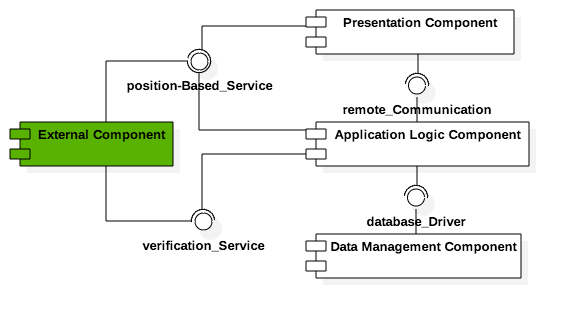
\includegraphics[width=\textwidth]{images/high_level_CD}
  	    		\caption{High Level Component Diagram}\label{fig-high}
		\end{figure}
	\begin{itemize}
	
		\item \textbf{External Component}
		
		Thanks to the requirement analysis process, we have figured out two basic expected functionalities provided by external system, which are position-based service and document verification service. So in the high-level component view, these two services are provided by an high-level component, \textsl{External Component}, with specific interface. 
		
		\item \textbf{Presentation Component}
		
		As we have decided in the RASD document, our system will offer two GUI to the user for visualizing the interaction. One of them is the mobile phone application and the other is the on-board application. These two perform a similar role in the overall system , so we combine them as one high-level component, \textsl{Presentation Component}. 
		
		This component uses the position-based service provided by the \textsl{External Component}, in order to visualize the position of user and car on a geographic map.
		Meanwhile, this component depends on the interface provided by the \textsl{Application Logic Component}, for the aim of interacting with the server.
		
		\item \textbf{Application Logic Component}
		
		This high-level component essentially represents all the business logic offered by our system.
			
		It provides logic response to \textsl{Presentation Component} with the help of \textsl{remote\_Communication} interface.
		 And it accesses to database by using the interface offered by the \textsl{Data Management Component}.
		
		\item \textbf{Data Management Component}
		
		This high-level component handles all the data related manipulation, and offers a driver interface for other components to access data. 
	\end{itemize}	 
		
	\subsection{Component view}
	After an overall looking of our system, now we are going to provide more details for the architecture with a low-level component view, which is shown in the Figure~\ref{fig-low}. The components here can be seen as the subcomponent of those in high-level view, and are described in detail as follows:
	 
		\begin{figure}[H]
   			\centering
   			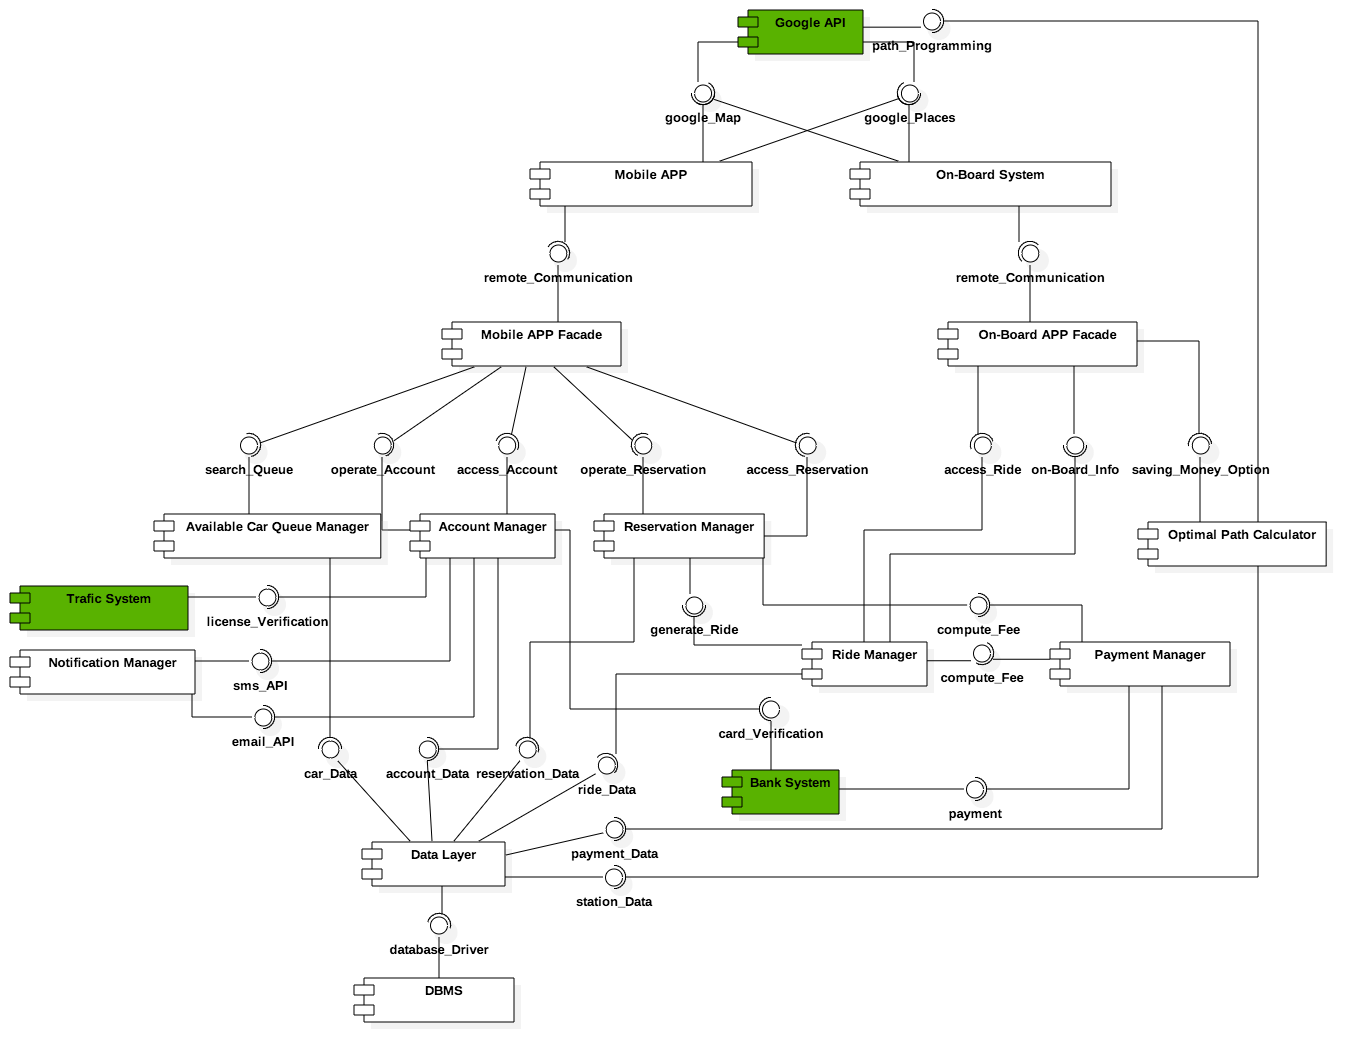
\includegraphics[width=\textwidth]{images/low_level_CD}
  	    		\caption{Low Level Component Diagram}\label{fig-low}
		\end{figure}
		\begin{itemize}
			\item \textbf{Google API} 
			
It is an external Google component that provides the \textsl{Mobile APP} and \textsl{On-Board system} some interfaces, makes the \textsl{PowerEnJoy} system able to get the data about information from the same database of \textsl{Google Maps}, also the geographical location of points from the same database of \textsl{Google+Local}.
			
			\item \textbf{Traffic System}
			
It is an external component that provides the \textsl{Account Manager} an interface, in order to make the \textsl{PowerEnJoy} system verify drive license by using data from the \textsl{Traffic system} database.

			\item \textbf{Bank System}
			
It is an external component that provides the \textsl{Account Manager} some interfaces, makes \textsl{PowerEnJoy} system be able to verify the credit card by using data from the database of banks.

			\item \textbf{Mobile APP}

It is the component which embeds on the mobile devices of users, it offers user a GUI that:
			\begin{itemize}
				\item Allows the users to access the functionality the system provide him.
				\item Displays the data obtained by the interaction with \textsl{Mobile APP Facade}.
			\end{itemize}
And it charges not only the presentation behaviours but also the communication duty in order to deliver the tasks user required as well as the message, and the response from \textsl{Mobile App Facade}.

			\item \textbf{On-Board System}
			
It is the component which is embedded inside the panel of the car, it offers a GUI that:
			\begin{itemize}
				\item Allows the users to access the functionality the system provide him to the car.
				\item Displays the data obtained by the interaction with \textsl{On-Board System Facade}.
			\end{itemize}
And this component can also handle all communications with the \textsl{On-Board System Facade} to accomplish the tasks. All messages from \textsl{On-Board System} to the \textsl{PowerEnJoy} servers are also from this component.

			\item \textbf{Mobile APP Facade}
			
This is a component implementing a \textsl{Facade Pattern}: this component offers the interfaces to accomplish the functionality that should be manipulated correspondingly by different managers. Only this facade has an interface which can interact with the \textsl{Mobile App}.

			\item \textbf{On-Board System Facade}
			
This is also a component implementing a \textsl{Facade Pattern}: this component offers the interfaces to accomplish the functionality that should be manipulated correspondingly by different managers. Only this facade has an interface which can interact with the \textsl{On-Board System}.

			\item \textbf{Available Car Queue Manager}
			
This component is able to access to the \textsl{Data Layer} component to get the car state information, and the manager updates the available cars as soon as the car state in \textsl{Data Layer} changes.

			\item \textbf{Account Manager}
			
It is the component which support the functionalities about registration and login. In order to do this, the Account Manager is able to:
			\begin{itemize}
				\item Access the external \textsl{Traffic System} component to verify the data.
				\item Access the external \textsl{Bank System} to verify the data.
				\item Access the \textsl{Notification Manager} to exchange messages.
				\item Access the \textsl{Data Layer} to store user data as well as check the history record.
			\end{itemize}

			\item \textbf{Reservation Manager}
			
This component handles reservation by:
			\begin{itemize}
				\item Access the \textsl{Data Layer} component in order to check or change the state of reservation.
				\item Make a countdown as well as get an reservation.
				\item Access the \textsl{Payment Manager} only if the reservation fails.
				\item Access the \textsl{Data Layer} component in order to change the car state as well as store reservation information.
				\item Access the \textsl{Ride Manager} only if the user picks up the car successfully.
			\end{itemize}
			
			\item \textbf{Ride Manager}
			
This component handles the car which is picked up successfully, it accesses to the \textsl{Reservation Manger}, commence the operation by the trigger of the message from Reservation Manager,and the \textsl{On-Board System} is triggered at the same time. The \textsl{Ride Manager} access the \textsl{On-Board System} and supply the functionality the user can get on aboard.

The \textsl{Ride Manager} accesses to the \textsl{Data Layer} at the end of the ride in order to update the car state as well as store the ride information,also accesses to the payment manager to transmit the payment information.

			\item \textbf{Payment Manager}	
			
It can receive the payment information by accessing the \textsl{Reservation Manager} and \textsl{Ride Manager}, after calculate the accurate money, the \textsl{Payment Manager} accesses to \textsl{Bank System} to get the money, and also accesses to the \textsl{Data Layer} to store the payment details.
		
			\item \textbf{Notification Manager}
			
It handles the text message and email which sent by the \textsl{PowerEnJoy} system to the users.

			\item \textbf{Optimal Path Calculator}
			
This component accesses to the \textsl{On-Board System} in order to get the address information from uses, and also able to access both the \textsl{Google API} and \textsl{Data Layer} to calculate the optimal path from start point to destination.

			\item \textbf{Data Layer}
			
			This is the component that allows \textsl{Reservation Manager}, \textsl{Account Manager}, \textsl{Available Car Queue Manager} ,\textsl{Ride Manager},\textsl{Optimal Path Manager} and \textsl{Payment Manager} to access the data which stored in database.

			\item \textbf{DBMS}
It is a external component that is able to interact with the database where all the system data are stored via query.
		\end{itemize}
	\subsection{Component interfaces}
	
In this part, we are going to give a detail description for the interfaces offered by components presented in the Low Level Component Diagram. Also we will describe how these interfaces help components to interacted with each other.
		\subsubsection{Google API}
			\begin{itemize}
				\item \textbf{google\_Map}

This interface provides three basic functions:
				\begin{itemize}
					\item a graphical representation of geographical maps
					\item the service of searching a particular address
					\item estimate the distance between two specified location 
				\end{itemize}

It is used by two other components listed as follows:
				\begin{itemize}
					\item \textsl{Mobile APP}: 
					
					The interface provides a graphical map for the mobile phone application, in order to visualize the position detected by the GPS, or alternatively the position with a specified address inserted by the user. 
					\item \textsl{On-Board System}: Similar to the component above, the interface provides a graphical map for the on-board application to display the current position of the car detected by GPS. Meanwhile, it enable the on-board application to search a particular address inserted by the user. 
				\end{itemize}
					
				\item \textbf{google\_Places}

This interface provides the service of searching marked position located around a given address. 

It is used by two other components listed as follows:
				\begin{itemize}
					\item \textsl{Mobile APP}: Together with the available car position data, this interface enable the mobile phone application to present position of available cars close to the user's location or an address specified by the user. 
					\item \textsl{On-Board System}: Together with the power station position data, this interface enable the on-board application to get position info of stations closed to the user's input destination. 
				\end{itemize}
 
				\item \textbf{google\_path\_Programming}	

This interface provides the service of programming a path between two specified position.			
It is used by the \textsl{Optimal Path Calculator} component, for the aim of programming an optimal path for those users whose select the "saving money option".
			\end{itemize}
			
		\subsubsection{Traffic System}
			\begin{itemize}
				\item \textbf{license\_Verification}

This interface provides the service of verifying a driving license, with the driving license ID offered by the user. Thanks to this, the assumption that all the users have a valid driving license is satisfied. 

It is used by the \textsl{Account Manager} when a new user tries to create an account.
			\end{itemize}
			
		\subsubsection{Bank System}
			\begin{itemize}
				\item \textbf{card\_Verification}

This interface provides the service of verifying a credit card, with the card number offered by the user. With the help of this, the assumption that all the users have have a credit card which can be used for the payment is satisfied.

It is used by the \textsl{Account Manager} when a new user tries to create an account, or whenever the user is willing to modify the card for payment
				\item \textbf{payment}
			\end{itemize}
	
		\subsubsection{Mobile APP Facade}
			\begin{itemize}
				\item \textbf{remote\_Communnication}

This interface provides access to all the functionalities, the mobile phone application offered to user, via proprietary protocols.

It is used by \textsl{Mobile APP} component to transfer the user's action to the logical layer, as well as transfer the logical result back to the user. 					
			\end{itemize}
			
		\subsubsection{On-Board System Facade}
			\begin{itemize}
				\item \textbf{remote\_Communication}

This interface provides access to all the functionalities, the on-board application offered to user, via proprietary protocols.

It is used by \textsl{On-Board System} component to transfer the user's action to the the logical layer, as well as transfer the logical result back to the user.
				
				\item \textbf{on-Board\_Info}

This interface provides access to car state data which is detected by the sensors on the car and sent from the \textsl{On-Board System} component. 

It is used by the \textsl{Ride Manager} to:
				\begin{itemize}
					\item count number of passengers
					\item modify ride state according to engine state
					\item detect battery level
					\item detect charging state
					\item detect parking position
				\end{itemize}
			\end{itemize}
			
		\subsubsection{Available Car Queue Manager}
			\begin{itemize}
				\item \textbf{search\_Queue}

This interface provides access to data of available cars.

It is used by the \textsl{Mobile APP Facade} component, when: 
					\begin{itemize}
						\item the user starts searching available cars; 
						\item the user selects one of the available to check detail information.
					\end{itemize}
			\end{itemize}
			
		\subsubsection{Account Manager}
			\begin{itemize}
				\item \textbf{operate\_Account}

This interface provides the service of creating new account and modifying account data of specified user.

It is used by the \textsl{Mobile APP Facade} component when a new user tries to register in the system, or when the user tries to modify personal account data, including:
					\begin{itemize}
						\item changing password
						\item changing payment method
						\item changing contact information
						\item modifying personal data
						\item deleting previous ride records.
					\end{itemize}
					
				\item \textbf{access\_Account}

This interface provides access to personal account data.

It is used by the \textsl{Mobile APP Facade} component when the user tries to login an account and check personal account data, including:
					\begin{itemize}
						\item checking current payment method
						\item checking contact information setting
						\item checking personal data
						\item checking previous ride records.
					\end{itemize}
			\end{itemize}
			
		\subsubsection{Reservation Manager}
			\begin{itemize}
				\item \textbf{operate\_Reservation}

This interface provides the service of creating new reservation and modifying current reservation state.

It is used by the \textsl{Mobile APP Facade} component when the user tries to:
					\begin{itemize}
						\item make reservation, which means create a new reservation and set status to ACTIVE
						\item cancel reservation, which means change current reservation status to CANCELLED
						\item pick up the car, which implies change current reservation status to COMPLETE.
					\end{itemize}
					
				\item \textbf{access\_Reservation}

This interface provides access to current reservation data.

It is used by the \textsl{Mobile APP Facade} component when the user tries to check current reservation data, including:
					\begin{itemize}
						\item reservation count down
						\item position of reserved car.
					\end{itemize}
					
				\item \textbf{generate\_Ride}

This interface provides the service of generating a new ride once a user complete a reservation by picking up the reserved car.

It transfers the user data and car data of a complete reservation to the \textsl{Ride Manager} component.
				
				\item \textbf{compute\_Fee}

This interface provides the service of computing demurrage and cancelled fine according to reservation status.

It transfers the amount of fee generated by the reservation operation to the \textsl{Payment Manager} for the aim of completing the fee payment.
			\end{itemize}
			
		\subsubsection{Ride Manager}
			\begin{itemize}
				\item \textbf{access\_Ride}

This interface provides access to current ride data.

It offers the real-time basic consumption to the \textsl{On-Board APP Facade}.
				
				\item \textbf{compute\_Fee}

This interface provides the service of computing final ride consumption by integrating the:
					\begin{itemize}
						\item basic consumption regraded to riding duration
						\item discount 
						\item compensation 
					\end{itemize}					 

It transfers the amount of fee generated by the ride to the \textsl{Payment Manager} for the aim of completing the fee payment.
				
			\end{itemize}
			
		\subsubsection{Notification Manager}
			\begin{itemize}
				\item \textbf{sms\_API}

This interface provides the service of sending text message to user.

It is used by the \textsl{Account Manager} in order to send the login password, which is generated by the application server, back to the user via text message.

				\item \textbf{email\_API}

This interface provides the service of sending email to user.

It is used by the \textsl{Account Manager} in order to send the login password, which is generated by the application server, back to the user via email.

			\end{itemize}
			
		\subsubsection{Optimal Path Calculator}
			\begin{itemize}
				\item \textbf{saving\_Money\_Option}

This interface provides the service of finding the optimal position of final parking power station, according to the destination specified by the user, as well as programming the optimal path to get there for the aim of saving money.

It transfers the optimal solution to the \textsl{On-Board Facade} component.
			\end{itemize}
			
		\subsubsection{Data Layer}
			\begin{itemize}
				\item \textbf{car\_Data}

This interface provides the search operation related to car status data.

It is used by the \textsl{Available Car Queue Manager}.

				\item \textbf{account\_Data}

This interface provides the database operations related to account data, including 
					\begin{itemize}
						\item search
						\item insert
						\item modify
						\item delete (only for previous reservation and ride records)
					\end{itemize}

It is used by the \textsl{Account Manager}.

				\item \textbf{reservation\_Data}

This interface provides the 	database operations related to reservation data, including 
					\begin{itemize}
						\item search
						\item insert
						\item modify
					\end{itemize}		

It is used by the \textsl{Reservation Manager}.
	
				\item \textbf{ride\_Data}

This interface provides the 	database operations related to ride data, including 
					\begin{itemize}
						\item search
						\item insert
						\item modify
					\end{itemize}		

It is used by the \textsl{Ride Manager}.

				\item \textbf{payment\_Data}

This interface provides the 	insert operations related to payment data.

It is used by the \textsl{Payment Manager}.
				
				\item \textbf{station\_Data}

This interface provides the 	search operations related to power station data.

It is used by the \textsl{Optimal Path Calculator}.				
			\end{itemize}
			
		\subsubsection{DBMS}
			\begin{itemize}
				\item \textbf{database\_Driver}

This interface enable the interaction with the database.

It is used by the \textsl{Data Layer}. 
			\end{itemize}
			
	\subsection{Deployment view}
		\begin{figure}[H]
   			\centering
   			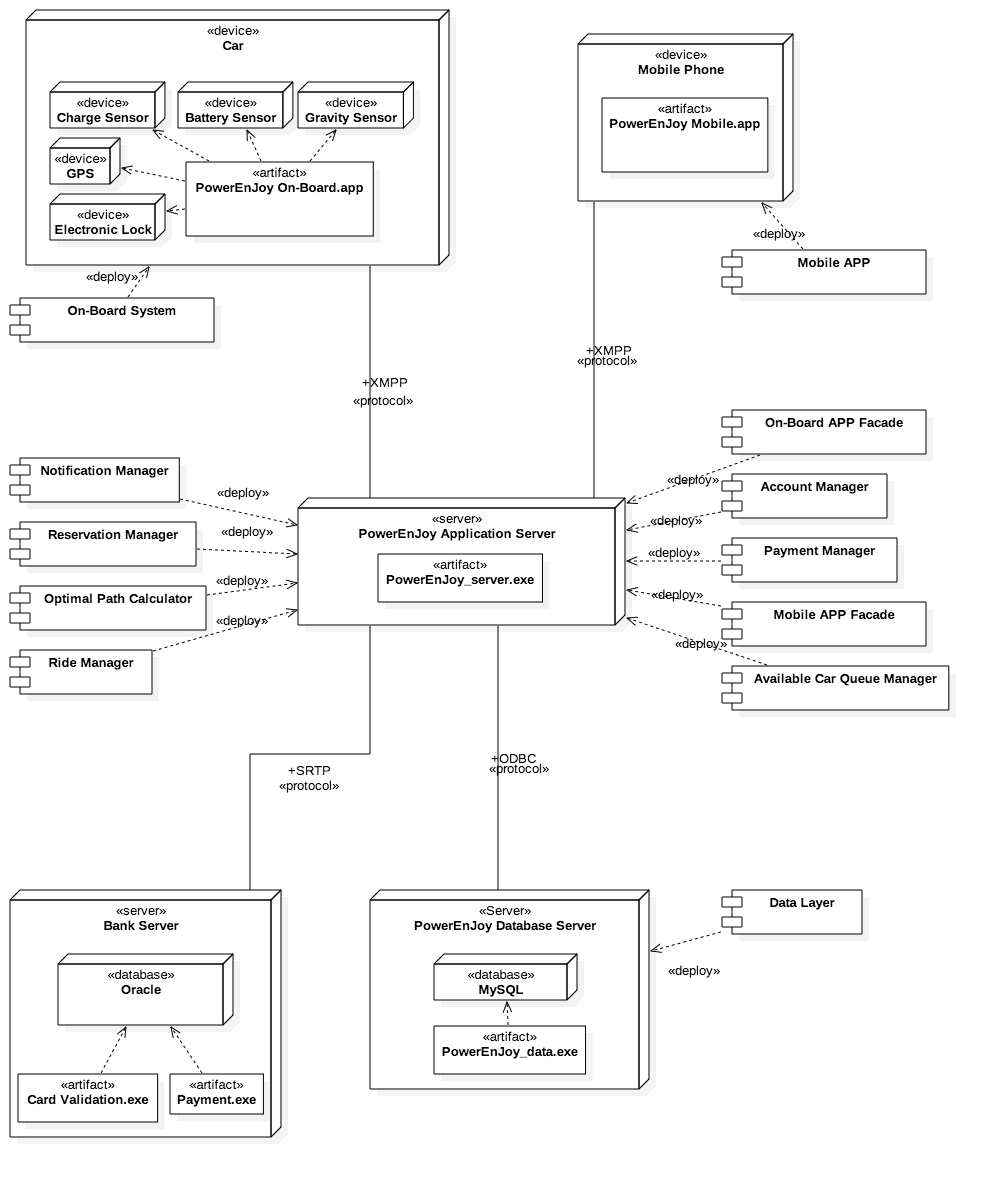
\includegraphics[width=\textwidth]{images/Deployment_View}
  	    		\caption{Deployment Diagram}\label{fig-deploy}
		\end{figure}

In the Figure~\ref{fig-deploy}, we present the hardware of the system, the sub-device deployed on the hardware, as well as the software that is installed on the hardware. In order to show the connection between component view and deployment view of our \textsl{PowerEnJoy} system, we also describe the deploy relation between each hardware and the logic components previously referred.

	\subsection{Runtime view}	
		\subsubsection{Register and Login}
The following Figure~\ref{fig-login} sequence diagram shows us how the component interact with each other when the \textsl{Mobile APP} get register and login request from the interface.

		\begin{figure}[H]
   			\centering
   			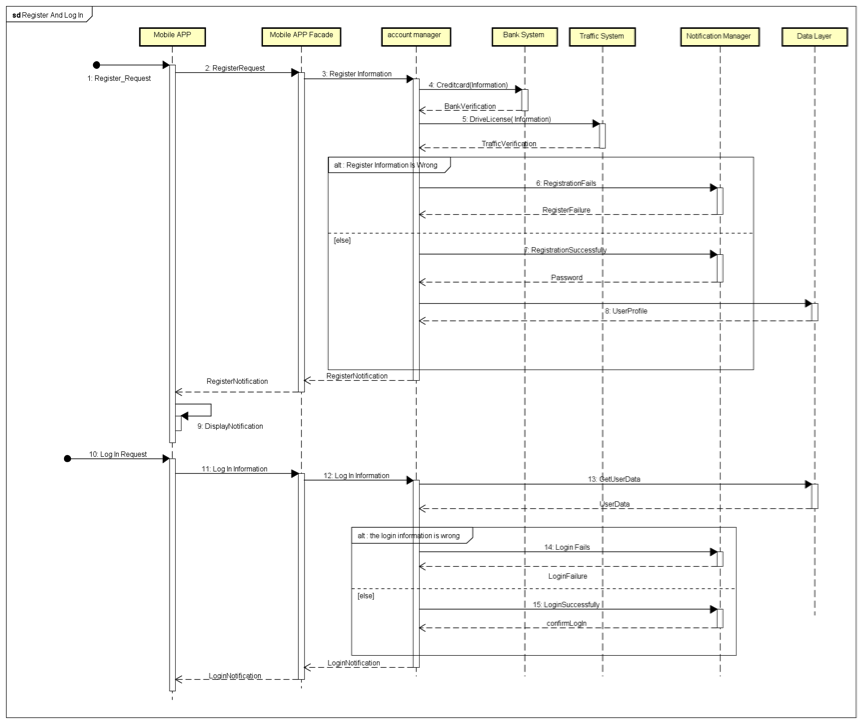
\includegraphics[width=\textwidth]{images/register_and_login_SD}
  	    		\caption{Register and Login}\label{fig-login}
		\end{figure}
		
Once guest accesses the \textsl{Mobile APP} and send a register request, the \textsl{Mobile APP} terminal gets the register information from the interface, then deliver it by remote server. The information flow through \textsl{Mobile APP Facade} and \textsl{Account Manager}, and be dispatched to the diverse external interfaces: \textsl{Traffic System} and \textsl{Bank System} in order to verify the availability. These two external interface both response a verification to \textsl{Account Manager}, the \textsl{Notification Manager} responses the different message corresponding to the verification result .If the guest register successfully, the register information will be stored in the database. Note that the profile stored also include the password system generated, and the guest can decide by himself if he should launch a new round of register under the condition of registration failed.

When the \textsl{Mobile APP} terminal gets the login request as well as the login information, it deliver the information to \textsl{Account Manager} through the \textsl{Mobile APP Façade} .The \textsl{Account Manager} checks the correctness of login information, then the \textsl{Notification Manager} responses messages corresponding to the check result. Note that the user can decide if he should launch a new round of login request under the situation of login failed. 
		
		\subsubsection{Make a Reservation}
The sequence diagram Figure~\ref{fig-makeres} shows how components interact with each other to make a reservation from the \textsl{Mobile APP} side.
		
		\begin{figure}[H]
   			\centering
   			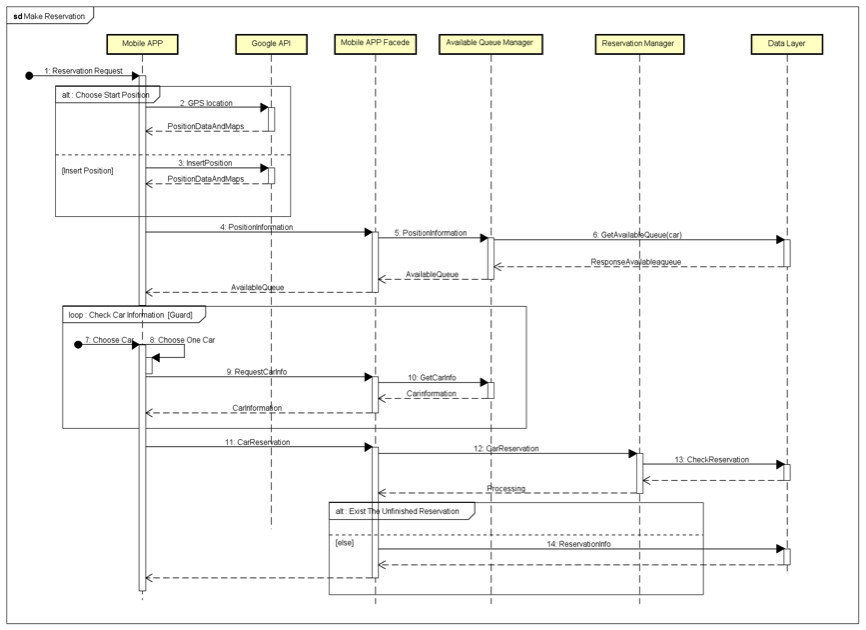
\includegraphics[width=\textwidth]{images/make_an_reservation_SD}
  	    		\caption{Make a Reservation}\label{fig-makeres}
		\end{figure}
		
User offers a start position, once the position be found, the \textsl{Google API} send back the position data and map around the start position to \textsl{Mobile APP} terminal, and also deliver the position information to \textsl{Mobile APP Façade} ,which trigger the execution of searching an available queue of car.

The \textsl{Available Car Queue Manager} then responses a queue to the \textsl{Mobile App} terminal, so that user can make reservation. The car will be removed from the available queue as long as it is reserved. The reservation data will be created in the database as well.

		\subsubsection{Cancel Reservation Automatically}
In this sequence diagram Figure~\ref{fig-cancelaut}, we can see how the reservation be cancelled automatically by system.

		\begin{figure}[H]
   			\centering
   			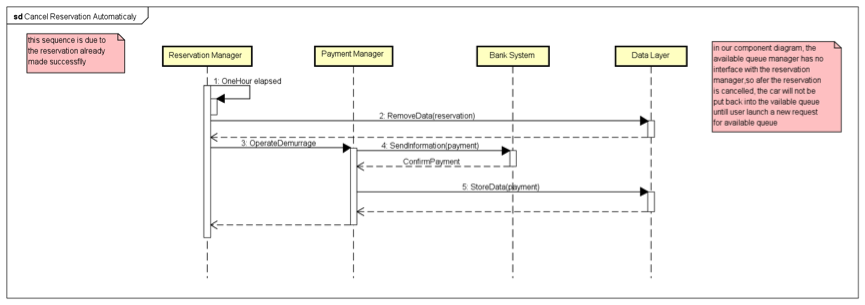
\includegraphics[width=\textwidth]{images/cancel_reservation_automatically_SD}
  	    		\caption{Cancel Reservation Automatically}\label{fig-cancelaut}
		\end{figure}
		
An hour elapse can trigger the Reservation Manager to cancel the current reservation; the \textsl{Payment Manager} should also interact with \textsl{Bank System} consequently to deduce the money as the compensation fee.

Note that the user can get the notification of reservation cancelled from the \textsl{Mobile APP} terminal.

		\subsubsection{Cancel Reservation Manually}
This following sequence diagram Figure~\ref{fig-cancelman} tell us how the component work together to let user cancel the reservation from \textsl{Mobile APP} terminal.

		\begin{figure}[H]
   			\centering
   			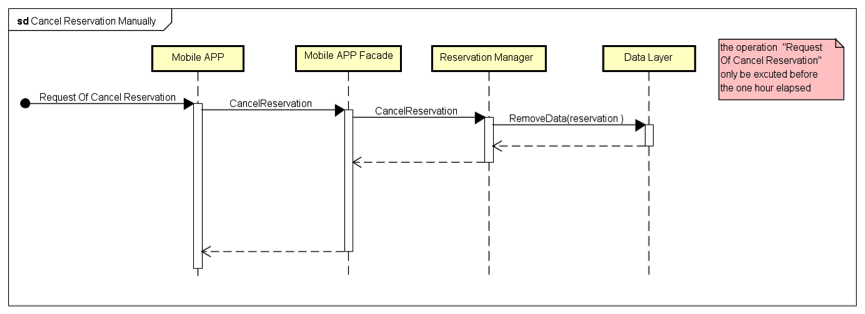
\includegraphics[width=\textwidth]{images/cancel_reservation_manually_SD}
  	    		\caption{Cancel Reservation Manually}\label{fig-cancelman}
		\end{figure}
		
The user launch a request to cancel the current reservation, the request is passed from remote server to the \textsl{Reservation Manager}, which removes the corresponding data from database and response the confirmation back. 

Note that this event can only exists when the reservation lives less than one hour, and the available queue will be updated when user launched a research of available queue.
		
		\subsubsection{Complete Ride on Mobile APP Side}
We can know from the following sequence diagram Figure~\ref{fig-completemob} about how the components cooperate together to accomplish a complete ride on the Mobile APP side.

		\begin{figure}[H]
   			\centering
   			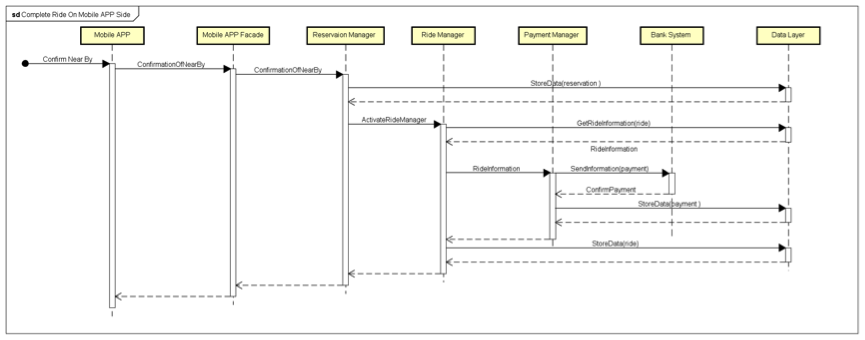
\includegraphics[width=\textwidth]{images/complete_ride_on_mobile_app_side_SD}
  	    		\caption{Complete Ride on Mobile APP Side}\label{fig-completemob}
		\end{figure}
		
This operation is mainly focuses on the messages exchange and data exchange between components, the step is:
			\begin{itemize}
				\item The user triggers the ride operation by a confirmation, the \textsl{Mobile APP} sends the confirmation by remote server, and activates the \textsl{Reservation Manager}. The \textsl{Reservation Manager} ends current reservation a successful finished reservation; store the information into the database. 
				\item The \textsl{Ride Manager} is ignited, the \textsl{Data Layer} responses the ride information back as well as the complete ride finished, the \textsl{Payment Manager} will calculate the accurate money that cost in the current ride.
				\item The \textsl{Payment Manager} sends the payment information to \textsl{Bank System}, which responses the confirmation of payment which signs the complement of payment. Then \textsl{Payment Manager} stores the payment data.
				\item The \textsl{Ride Manager} stores the data, and the whole system response step-wisely.
			\end{itemize}	
			
Note that the ride operation is executed in the same time at both the \textsl{Mobile APP} side and the \textsl{On-Board System side}, the ride is completely finished only if the executions finished in both side. These two sides have data communication, which is not showed in this sequence diagram.	

		\subsubsection{Complete Ride on On-Board System}		
In the following sequence diagram Figure~\ref{fig-completebod} ,we can see the ride operation details on the \textsl{On- Board System} side.	

		\begin{figure}[H]
   			\centering
   			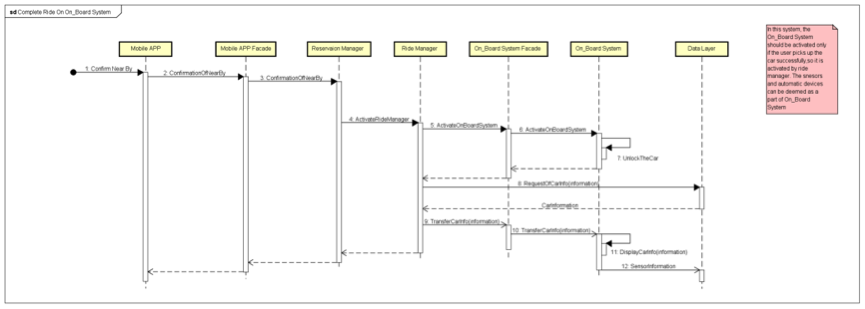
\includegraphics[width=\textwidth]{images/complet_onboard}
  	    		\caption{Complete Ride on On-Board System}\label{fig-completebod}
		\end{figure}
		
The \textsl{On-Board System Facade} is activated by the Ride Manger, then the \textsl{On-Board System} is activated consequently. The \textsl{On-Board System} terminal unlocks the car, and it signify the start of a ride.

The \textsl{Ride Manager} get the car information, then the \textsl{On-Board System} terminal displays the information on the screen. the \textsl{On-Board System} also send the sensor information to the \textsl{Data Layer} asynchronously.

Note that the \textsl{On-Board System} include all the sensor embedded into the car, the display screen, the GPS, also the autonomic devices like the lock in the door. The \textsl{On-Board System} sends the car information real-timely to the \textsl{Data Layer}. The accomplishment of a complete ride is also gained from the sensors information.

		\subsubsection{Saving Money Option}
In the last sequence diagram Figure~\ref{fig-saving}, we can know exactly how the component work together, supplies the way to users to access the saving money option.
		
		\begin{figure}[H]
   			\centering
   			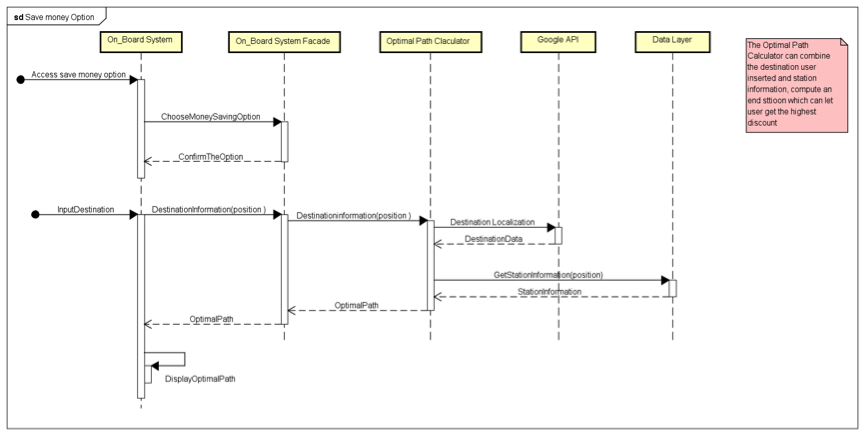
\includegraphics[width=\textwidth]{images/saving_money}
  	    		\caption{Saving Money Option}\label{fig-saving}
		\end{figure}
The request is received from the interface of \textsl{On-Board System}. When the \textsl{On-Board System} confirms the request successfully, the \textsl{On-Board System} will have the interface to get the destination information from user.

The \textsl{On-Board System Facade} sends the destination information to the \textsl{Optimal Path Calculator}; the \textsl{Optimal Path Calculator} gets the destination data from \textsl{Google API}, the station information from the \textsl{Data Layer}, and responses the optimal path to the fittest station.

The optimal path is returned to the \textsl{On-Board System} and be showed on the screen.

Note that the station information also includes the information of plugs sensor in the power station, so that the \textsl{Optimal Path Calculator} can also consider the free plugs in that power station.
		
	\subsection{Selected architectural styles and patterns}
		\begin{figure}[H]
   			\centering
   			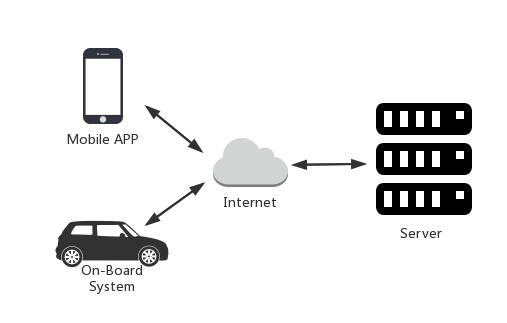
\includegraphics[width=\textwidth]{images/Client_Server}
  	    		\caption{Client-Server Architecture Style}\label{fig-style}
		\end{figure}
		
		\subsubsection{Architectural style}
As it is shown in Figure~\ref{fig-style}, our system is basically based on \textsl{client-server} architecture style. And there are two types of clients connected to the server. According to the system feature, we choose to use 3-tier architecture to deploy our system. The physical architecture is presented in Figure~\ref{fig-tier}. In the following two paragraphs we will explained the two different types of clients in detail.	
		
			\begin{itemize}
				\item \textbf{Mobile Application Client} 
				
				The Mobile Application is a \textsl{thin} client, because the business logic is implemented entirely one the application server. This client provides a presentation layer for the user to manipulate data related to personal account, current reservation, and previous records. Also it can deliver the response of application server to user by displaying them on the mobile phone screen. So basically this client represents a GUI.

		\begin{figure}[H]
   			\centering
   			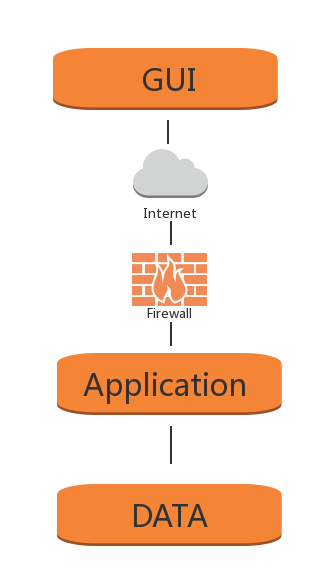
\includegraphics[width=0.4\textwidth]{images/3z_Tiers_Architecture}
  	    		\caption{3-Tier Architecture}\label{fig-tier}
		\end{figure}
						
				\item \textbf{On-Board System Client} 
				
				The On-Board System is also \textsl{thin} client, because it transfers all the car status information to the application server, which actually executes the business logic. This client provides a GUI for user who has successfully picked up a car; allows the user to select \textsl{saving money option}; and displays the current basic consumption on the on-board screen. 
			\end{itemize}				
		\subsubsection{Design patterns}
			\begin{itemize}
				\item \textbf{MVC Pattern}
				
					For the entire software structure, we use MVC pattern, which stands for Model-View-Controller Pattern. This pattern is used to separate application's concerns. In our project:
					\begin{itemize}
						\item View lies on both two client side, to handle the interaction with users.
						\item Model and Controller are deployed on the server side, for the aim of maintaining business logic and dealing with data manipulation. 
					\end{itemize}
				
				\item \textbf{Facade Pattern}
					For the structure of server side, we use Facade pattern to hide the complexities of the system and provide an interface to the client using which the client can access the system. We implement this pattern by simply adding to facade components:\textsl{Mobile APP Facade} and \textsl{On-Board System Facade}.
					
			\end{itemize}
		
	\subsection{Other design decisions}
	\subsubsection{Database Design}
	In this paragraph we report an ER diagram that describes the structure of \textsl{PowerEnJoy} database.
	\begin{figure}[H]
   			\centering
   			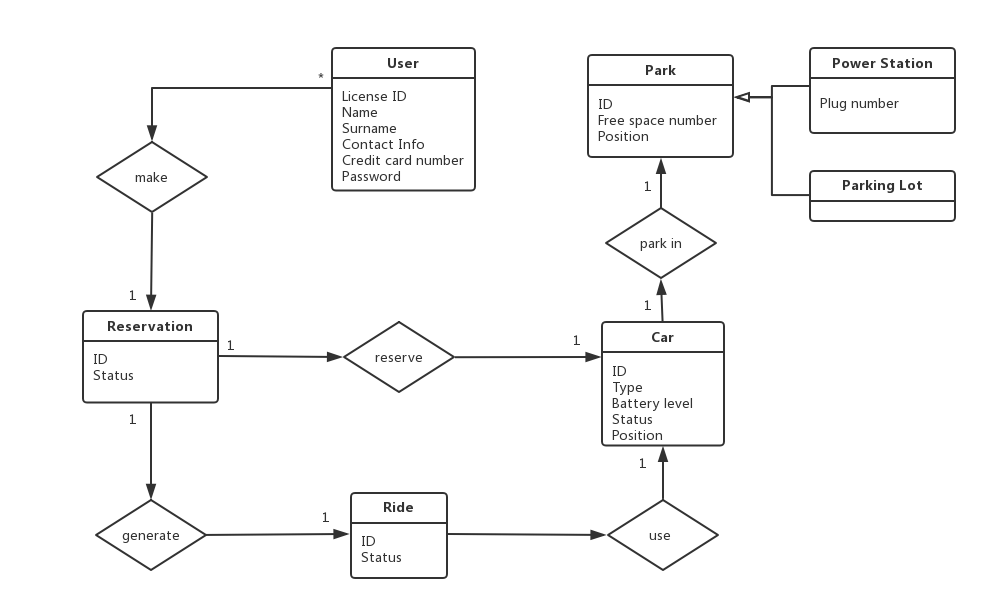
\includegraphics[width=\textwidth]{images/ER}
  	    		\caption{E-R Diagram}\label{fig-ER}
		\end{figure}
	\subsubsection{Programming Language}
	Considering the implementation of our \textsl{PowerEnJoy} system, we decide to use JAVA as our programming language. This is mainly because of Java's robustness, ease of use, cross-platform capabilities and security features. And our system shall be developed on the Java EE platform, which ensures us large-scale, multi-tiered, scalable, reliable, and secure properties.

\newpage
\section{ALGORITHM DESIGN}
For a clearer description about our project, we clarify the algorithm about queue management, pay management and money saving option, which we think they are important aspects of development of application.
	\subsection{Queue Management}
	This algorithm needs the position information about all the available cars in the city, as well as the accurate start position information from the user. Every time user launches a request for the available cars,the \textsl{Available Queue Manger} gets the coordinates of available cars in the city, then it starts the research of an available queue of cars around the start position which insert by user or oriented by GPS.

Cars in the queue will be updated when a new request of searching is launched. It can be added with the cars which is released from a ride or a reservation, it can also be removed by reservation.

Cars in the available queue are enumerated in the increase order in distance to the start position and the decrease order both in dump energy of car. The available car which is far than 3 KM are be consider as unreachable cars, and will not be enumerated in the available queue.

The research is done in according to the algorithm bellow, written in pseudo code:


\begin{lstlisting}[language={[ANSI]C}, frame=shadowbox]
Function searchAvailableQueue
cars(array)
destination(GPS coordinate)
while Distance(car.location,start)<=3
     Sort(
               cars as car;
               by  Distance(car.location,start)
               *10000000+(100-car.battery)
            )
     return cars;
End function

\end{lstlisting}

	\subsection{Payment Management}
	This algorithm needs the sensor information about both the car and power station. When a ride finished, the system sends all the sensor information to the \textsl{Payment Manager} in order to compute the money user should pay in this ride.

The computation is done in according to the algorithm bellow, written in pseudo code:
\begin{lstlisting}[language={[ANSI]C}, frame=shadowbox]
Function PaymentCalculate 
Sensor(array)
Discount1:=0.8
Discount2:=0.7
Compensation:=1.3
ComputeFinalPrice(
             price:=Sensor.rideTime*moneyPerMinute
             numPassengers:=Sensor.passenger
             dumEnery:=Sensor.battery
            if( numPassengers>2)
                price:=price*Discount1
            if( dumEnergy/fullBattery>0.5)
                price:=price*Discount1 
            if( dumEnergy/fullBattery<0.3)
                price:=price*Compensation
            if( numPassengers>2)
                price:=price*Discount
            if(Sensor.plug)
                price:=price*Discount2
            if(( Distance(car.location,powerStation))>3)
                price:=price*Compensation
)
return price 
End 
\end{lstlisting}
	\subsection{Money Saving Calculation}
	This algorithm is used for calculate the optimal station near the destination which user can get the height discount. It needs the destination from \textsl{On-Board System}, also the distribution of power station.The algorithm consider both the distance and the accessibility of power plugs, return user the optimal station not only reduce the cost of user but also contribute the cars in a reasonable way.
	
\begin{lstlisting}[language={[ANSI]C}, frame=shadowbox]
powerStation(array)
destination(GPS coordinate)
function moneySavingOption(powerStation,destination)
suggestedStation<-none
currentDistance<-infinite 
for ps in powerStations
   distance<-distance(destination,ps.location)
    if ps.numPowerPlugs>0 and (
         distance<currentDistance or(
             distance=currentDistance 
          and suggestedStation.numPowerPlugs
          	<ps.numPowerPlugs
                                 )
                            )
    then
       suggestedStation<-ps
       currentDistance<-distance
return suggestedStation
\end{lstlisting}
\newpage
\section{USER INTERFACE DESIGN}
In this section we discus about the design of two user interfaces with the help of mockups.
	\subsection{Mobile Application Interface}
	
	\begin{itemize}
\begin{figure}[H]
  \centering
  \begin{minipage}[t]{.35\linewidth}
    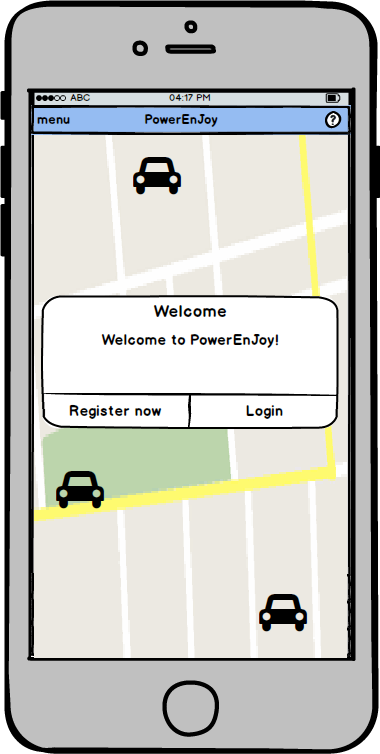
\includegraphics[width=\textwidth]{images/welcome}  
  \caption{Welcome Page}\label{fig-welcome}
  \end{minipage}
  \begin{minipage}[t]{.35\linewidth}
    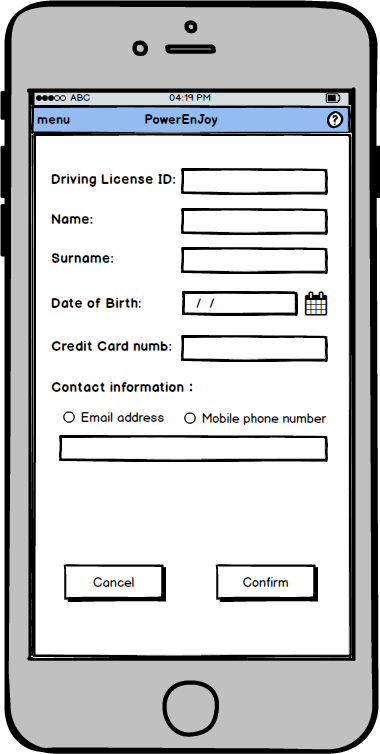
\includegraphics[width=\textwidth]{images/register}
  \caption{Register Page}\label{fig-register}
  \end{minipage}  
\end{figure}
	\item Figure~\ref{fig-welcome} shows the welcome page of our mobile application, which is presented to users once they open the APP. This page provides a register choice for new users, and offers a login choice for those users who already have an account.
	\item Figure~\ref{fig-register} simply gives the basic required information that user has to provide for the aim of registering in our system.
	
\begin{figure}[H]
  \centering
  \begin{minipage}[t]{.35\linewidth}
    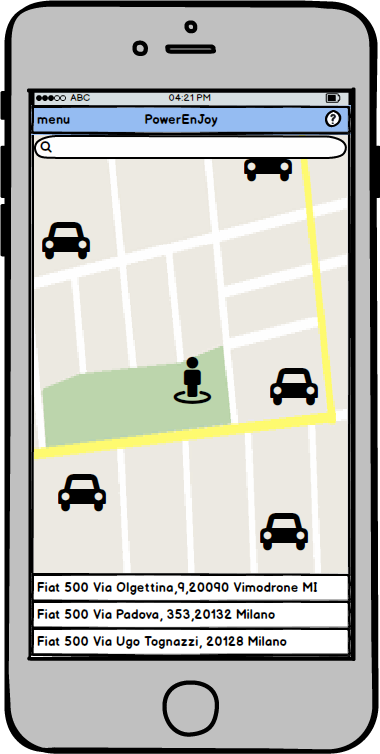
\includegraphics[width=\textwidth]{images/self}  
  \caption{Self Positioning}\label{fig-self}
  \end{minipage}
  \begin{minipage}[t]{.35\linewidth}
    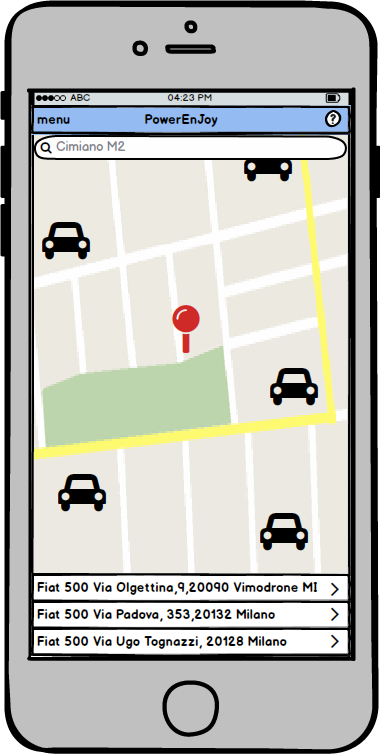
\includegraphics[width=\textwidth]{images/search}
  \caption{Search Position}\label{fig-search}
  \end{minipage}  
\end{figure}

	\item Figure~\ref{fig-self} presents the self-positioning, which is one of the two approaches to specify a position in order to search for available cars.
	\item Figure~\ref{fig-search} shows another method to search available car, which is to input a specific address.
	\item Figure~\ref{fig-make} is the page provided to user for making a reservation. In this page, user can check the basic information of the car to reserve, including car type, parking position, and battery level.
	\item Figure~\ref{fig-pick} shows the page for picking up the reserved car. In this page user is notified by the countdown of current reservation. This page is alive only within the one hour's countdown, and it will dead as soon as the reservation time up.
\begin{figure}[H]
  \centering
  \begin{minipage}[t]{.35\linewidth}
    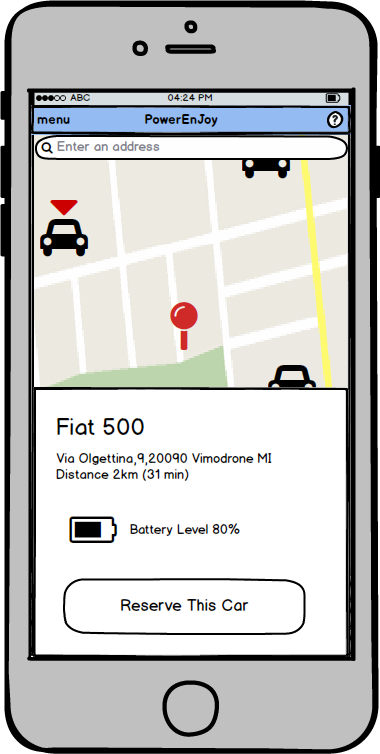
\includegraphics[width=\textwidth]{images/make}  
  \caption{Make Reservation}\label{fig-make}
  \end{minipage}
  \begin{minipage}[t]{.35\linewidth}
    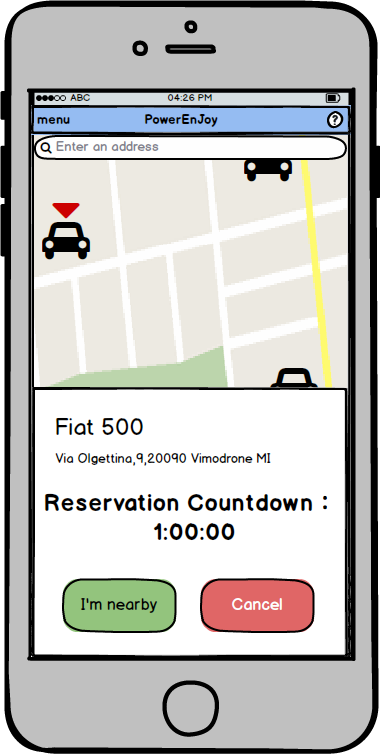
\includegraphics[width=\textwidth]{images/pick}
  \caption{Pick Up Car}\label{fig-pick}
  \end{minipage}  
\end{figure}	
	\end{itemize}

	\subsection{On-Board Application Interface}
	\begin{itemize}
	\item Figure~\ref{fig-desk} shows the desktop of our on-board application.It basically visualizes the essential information of a ride to user, including the current position of the car, real-time consumption, battery level, and ride duration. 
	\item Figure~\ref{fig-navigation} shows the page for user to input the destination. This page is triggered whenever the user press on the Navigation button or the Money Saving button.
	\item Figure~\ref{fig-path} presents the general navigation page provided to user who has not activated the money saving option. Here we can see that the destination is exactly the one that user specified.
	\item Figure~\ref{fig-optimal} shows the navigation page for user who has activated the money saving option. In this page, the final destination is calculated by our system according to the \textsl{Money Saving Calculation} algorithm.
	\item Figure~\ref{fig-nearby} presents the service of searching the power station closed to user. This is an additional service which has not been referred before, but it is quite simple to realize by using part of the logic of existed service. We offer it here to simplify the parking place finding process of our user. 
	\end{itemize}
	\begin{figure}[h]
   			\centering
   			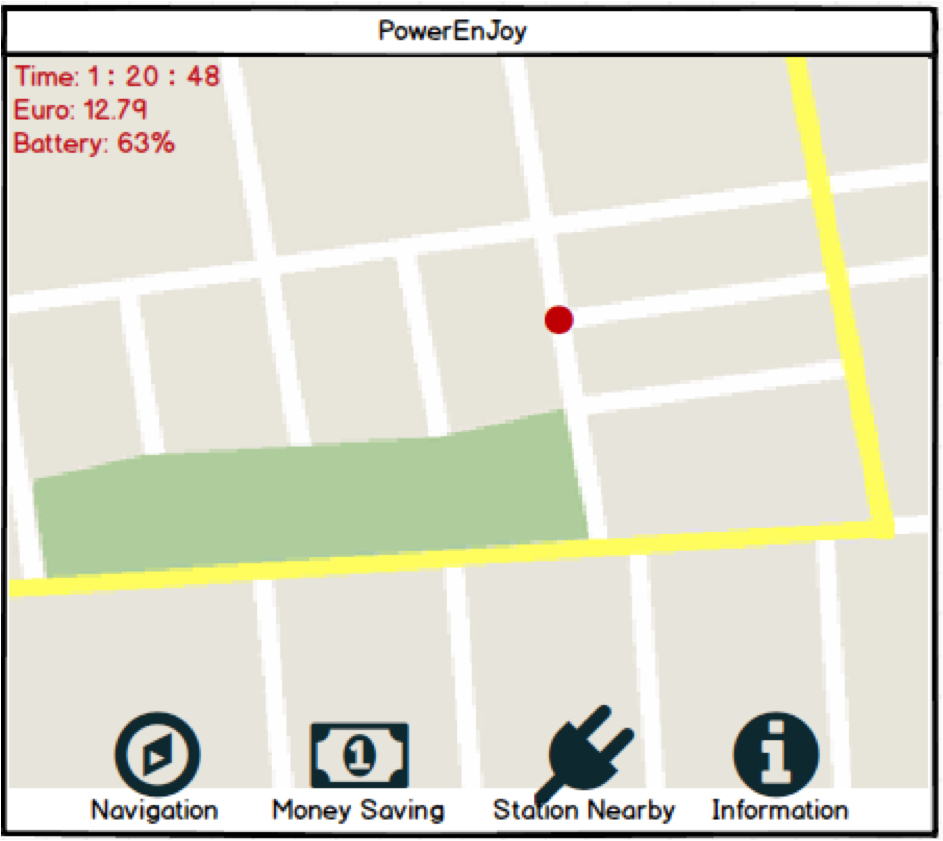
\includegraphics[width=0.8\textwidth]{images/desk}
  	    		\caption{On-Board Application Desktop}\label{fig-desk}
	\end{figure}
	\begin{figure}[H]
   			\centering
   			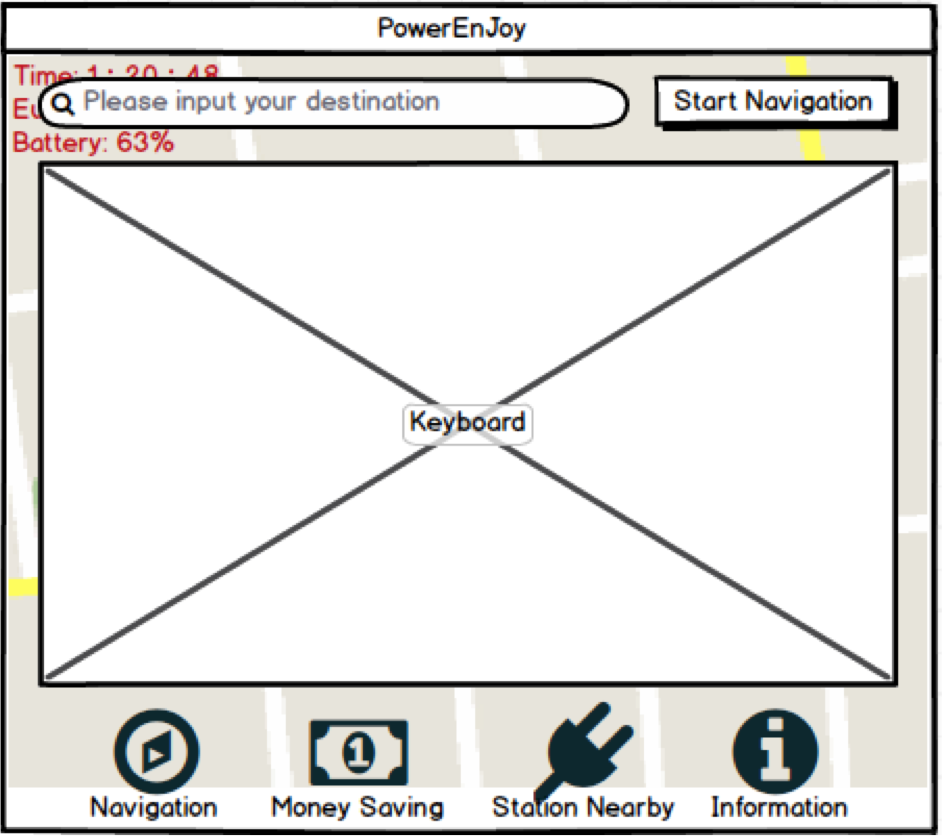
\includegraphics[width=0.8\textwidth]{images/navigation}
  	    		\caption{Input Destination}\label{fig-navigation}
	\end{figure}
	
	\begin{figure}[H]
   			\centering
   			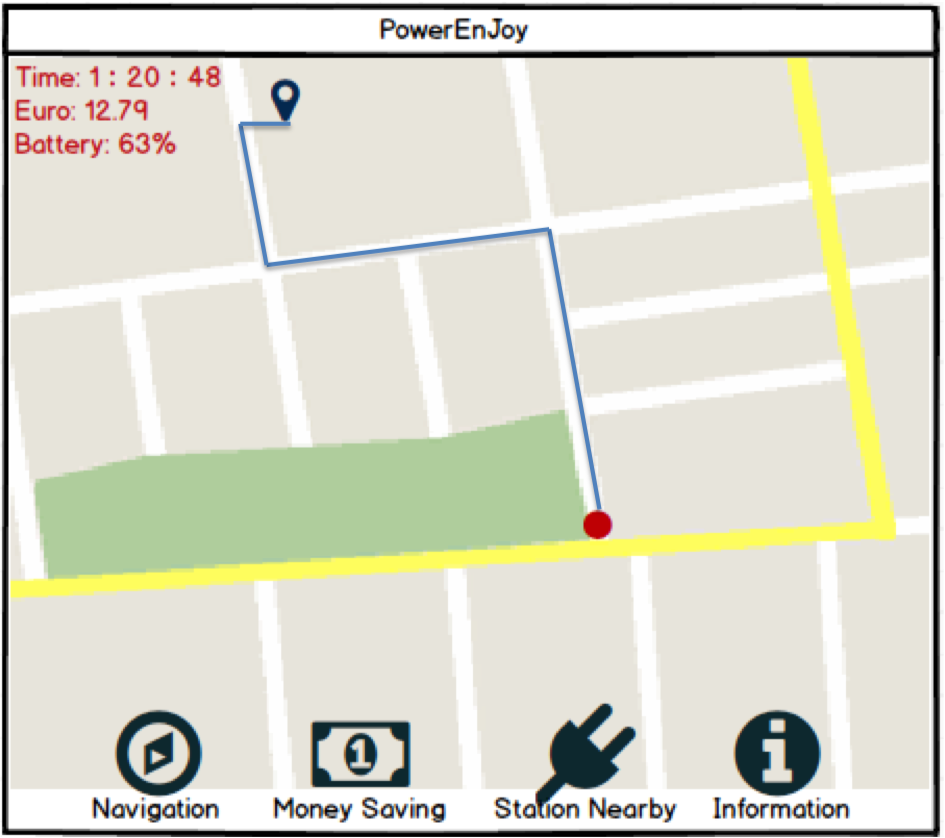
\includegraphics[width=0.8\textwidth]{images/path}
  	    		\caption{Navigation Path}\label{fig-path}
	\end{figure}
	
	\begin{figure}[H]
   			\centering
   			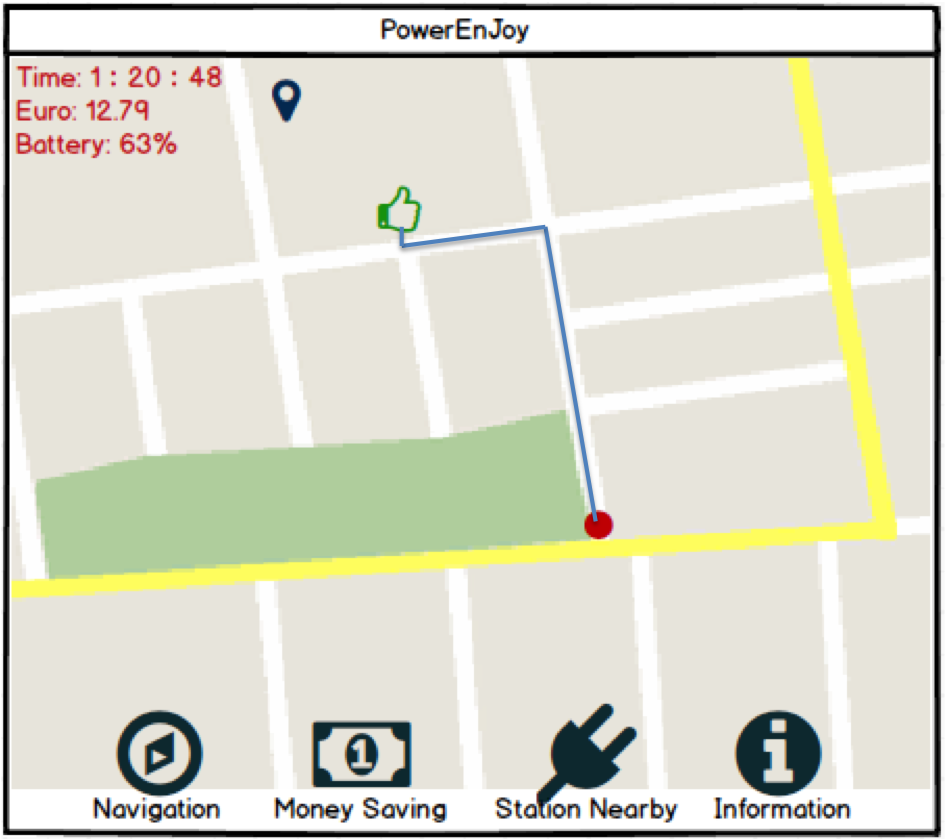
\includegraphics[width=0.8\textwidth]{images/optimal}
  	    		\caption{Money Saving Option}\label{fig-optimal}
	\end{figure}
	
	\begin{figure}[H]
   			\centering
   			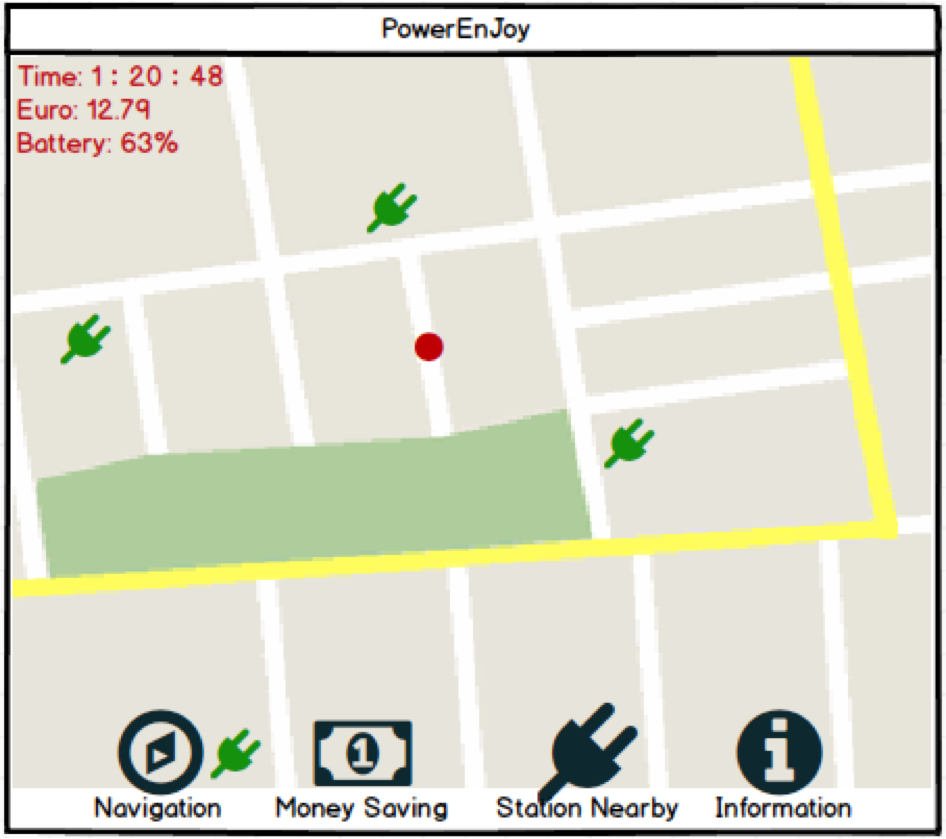
\includegraphics[width=0.8\textwidth]{images/nearby}
  	    		\caption{Search Power Station Nearby}\label{fig-nearby}
	\end{figure}

	
\newpage
\section{REQUIREMENTS TRACEABILITY}
In this section, we list the requirements specified in the previous RASD together with the components, which are designed in this document to assure its fulfillment.
\begin{center}
\renewcommand\arraystretch{2}
\begin{tabular}{|c|c|c|}
 \hline
Reference& Requirement& Component\\
 \hline
[1]& Register to be a user.& Account Manager \\
&&Bank System \\
&&Traffic System\\
 \hline
[2]& Get the notification about register. & Notification Manager \\
 \hline
 [3]& Login& Account Manager \\
 \hline
[4]& Search for available cars. & Available Queue Manager \\
&&Google API\\
 \hline
 [5]& Make a reservation.& Reservation Manager \\
 \hline
 [6]& Cancel reservation.& Reservation Manager \\
 \hline
 [7]& Check current reservation.& Reservation Manager \\
 \hline
 [8]& Pick up the car. & Mobile APP \\
&&Reservation Manager\\
 \hline
 [9]& Access the saving money option. & Google API \\
&&Optimal Path Calculator\\
&&On-Board System\\
 \hline
 [10]& Get the discount and compensation. & Payment Manager \\
 \hline
\end{tabular}
\end{center}
\newpage
\section{EFFORT SPENT}

\renewcommand\arraystretch{2}
\begin{tabular}{| p{5cm}| p{7cm}|}
 \hline
Gao Xiao& 50 Hours \\
 \hline
Kang Shuwen& 50 Hours \\
 \hline
Liubov Bolshakova& 30 Hours \\
 \hline

\end{tabular}

\newpage
\section{REFERENCES}
	\subsection{Reference Documents}
	\begin{itemize}
		\item Specification Document Assignments AA 2016-2017
		\item RASD
	\end{itemize}
	\subsection{Used Tools}
	The tools used to creat this document are:
	\begin{itemize}
		\item UMLStar: for UML models
		\item Github: for version control
		\item Latex: for typesetting
		\item Balsamiq: for mockup design
		\item ProcessOn: for network diagram
		 
	\end{itemize}

\newpage
	
\end{document}